\begin{frame}
\frametitle{Results in terms of Market Penetration Rate}
Spatial distribution of congestion is better achieved at higher \emph{penetration rates}, effects of works are better avoided. Nevertheless, increasing the \emph{penetration rate} may also have an impact on the \emph{network throughput}.
\begin{center}
\begin{columns}
    \begin{column}{0.3\textwidth}
    \begin{figure}
        \centering
        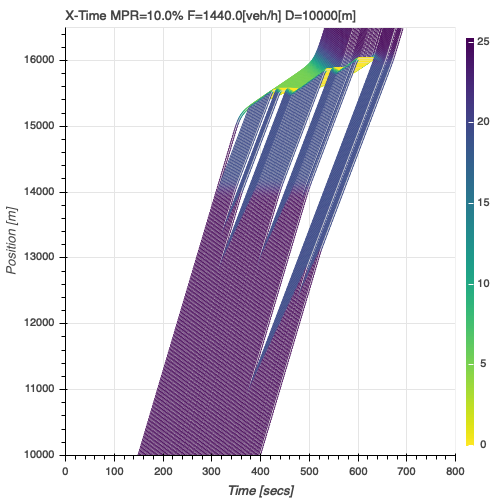
\includegraphics[width =1.15\textwidth]{fig_86_xt_mpr10}
        \caption{MPR = $10\%$}
    \end{figure}
    \end{column}
    \begin{column}{0.3\textwidth}
        \begin{figure}
            \centering
            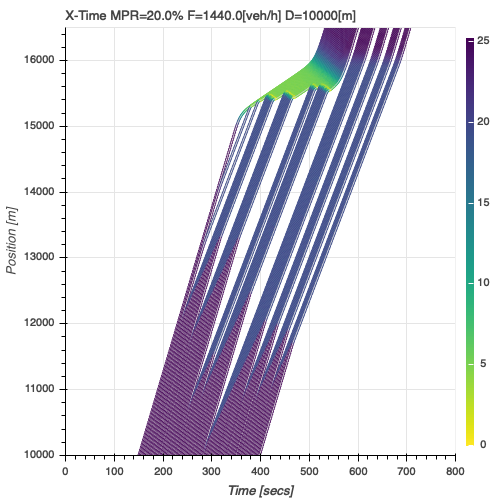
\includegraphics[width = 1.15\textwidth]{fig_87_xt_mpr20}
            \caption{MPR = $20\%$}
        \end{figure}
    \end{column}
    \begin{column}{0.3\textwidth}
        \begin{figure}
            \centering
            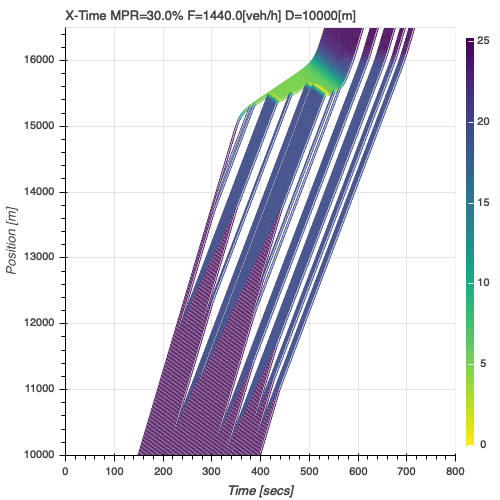
\includegraphics[width = 1.15\textwidth]{fig_88_xt_mpr30}
            \caption{MPR = $30\%$}
        \end{figure}
    \end{column}
\end{columns}
\end{center}
\end{frame}